
\section{Example Application Model}
\label{sec:example}

\begin{figure}[t]
\centering
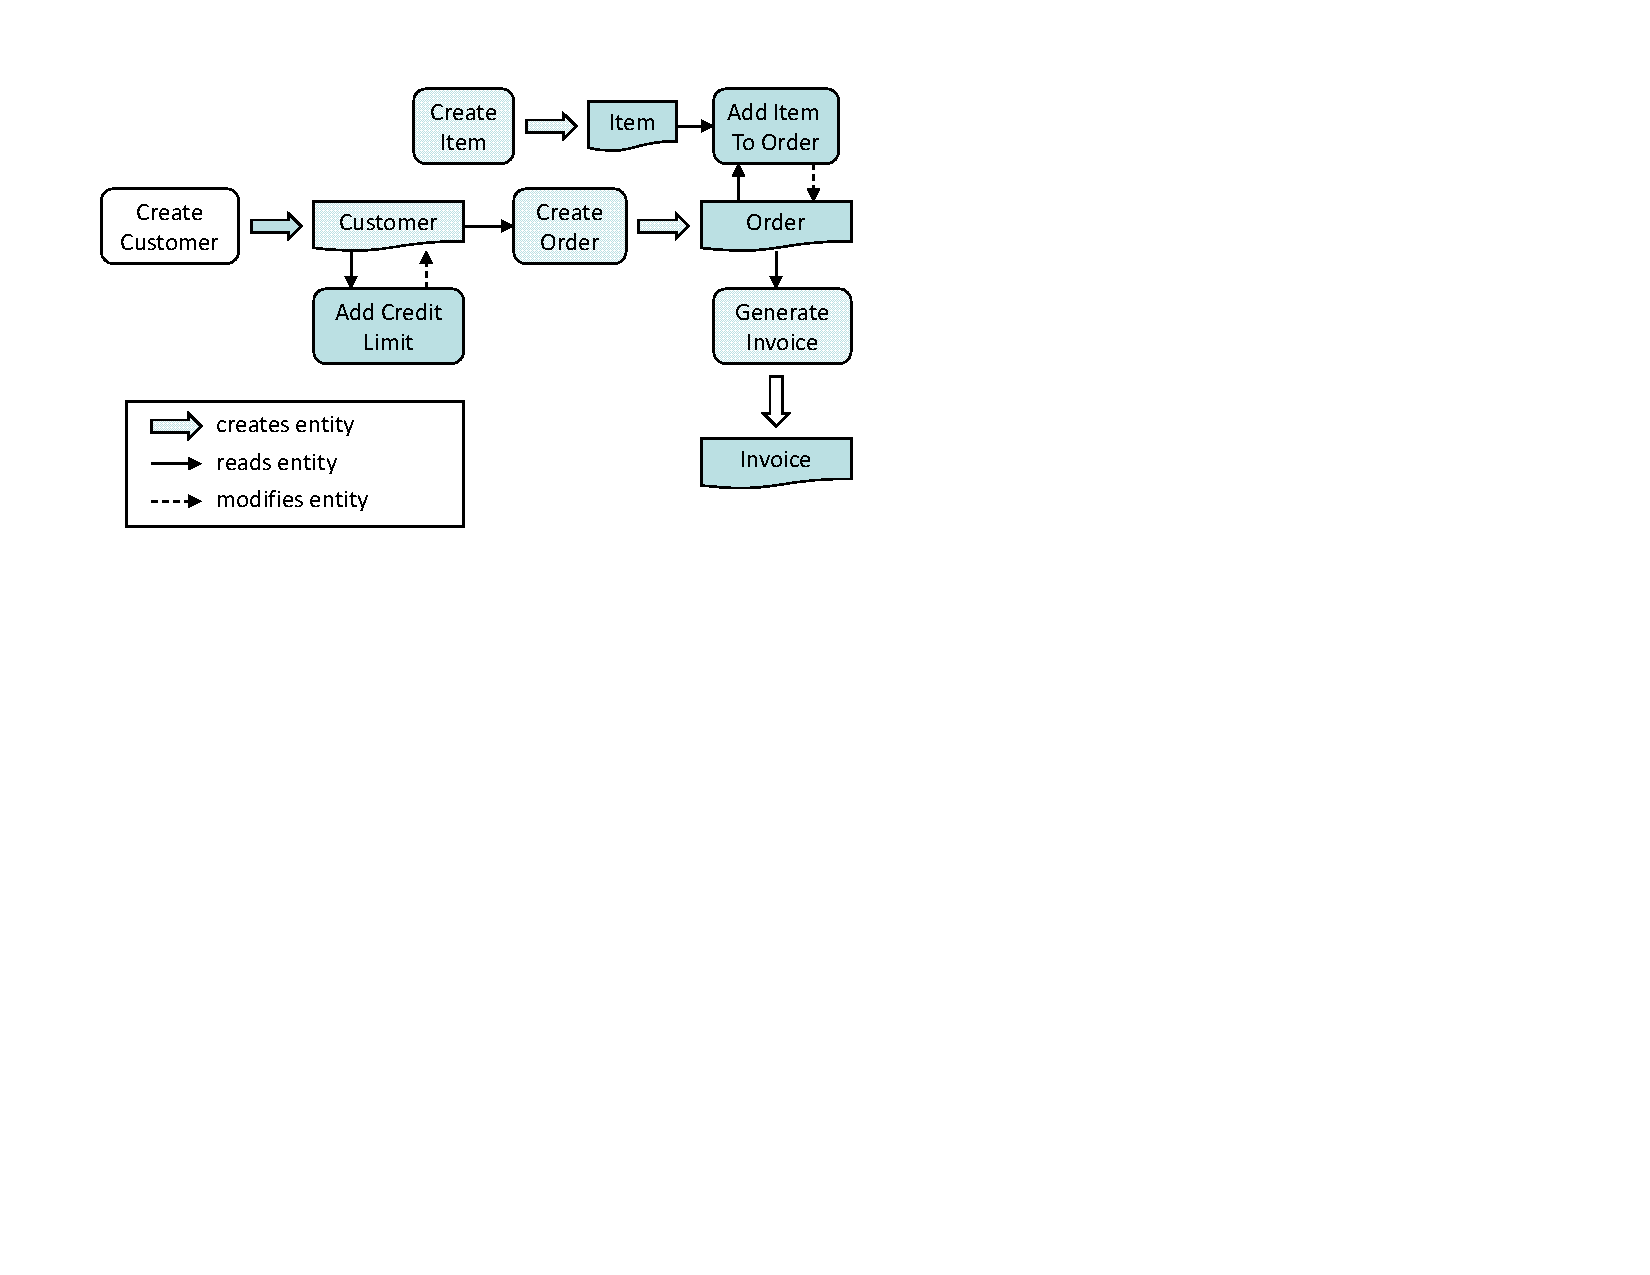
\includegraphics[trim=47 350 380 42,clip,width=\columnwidth]{figs/appModel.pdf}
\vspace*{-15pt}
\caption{Sample operations and their interactions in \subject{jBilling}.}
\vspace*{-12pt}
\label{fig:sample-app}
\end{figure}

Before presenting our technique, we elaborate upon the billing application
example (\subject{jBilling}) mentioned in the previous sections: we explain
various operations and rules for the application, which we use subsequently to
illustrate our technique. To facilitate the illustration, we use a simplified
version inspired by the actual application.\footnote{\scriptsize
  \url{http://www.jbilling.com/}} (In the empirical evaluation, we modeled a
larger part of the actual application.) The model for \subject{jBilling}
includes four entities: \subject{Customer}, \subject{Item}, \subject{Order}, and
\subject{Invoice}.  Figure~\ref{fig:sample-app} shows the flow among some of the
operations, which create and/or modify these entities. For example, operation
\subject{CreateCustomer} creates an instance of \subject{Customer}, whereas the
operation \subject{AddItemToOrder} modifies an \subject{Order} instance by
adding a new item to the order.

\begin{table*}[t]
\caption{Formal specification of sample business rules in \subject{jBilling}.}
\centering
\tabcolsep=4pt
{\scriptsize
\begin{tabular}{|l|l|l|l|l|l|}
\hline
& & & & \multicolumn{2}{|c|}{Rules $(R)$} \\
\cline{5-6}
\multicolumn{1}{|c|}{Operation} &
\multicolumn{1}{|c|}{Inputs $(I)$} &
\multicolumn{1}{|c|}{Creates $(C)$} &
\multicolumn{1}{|c|}{Modifies $(M)$} &
\multicolumn{1}{|c|}{Description} &
\multicolumn{1}{|c|}{Formal Representation} \\
\hline \hline
Create & \{{\tt State,} & \{{\tt Customer}\} &
\multicolumn{1}{|c|}{$\emptyset$} &
$R_1$: The \textit{credit limit (crLimit)} of newly  &
$r_{1.1}$: $({\tt true}) \Longrightarrow ({\tt cust.state} = {\tt state} \; \wedge$ \\
Customer & {\tt BalanceType}\} & & & created customers should be \textit{zero} &
\hspace*{10pt}$ {\tt cust.balType} = {\tt  balType} \; \wedge {\tt cust.crLimit} = 0)$ \\
\hline
Create & \{{\tt Int}\} & \{{\tt Item}\} & \multicolumn{1}{|c|}{$\emptyset$} &
$R_2$: The price of an item must be greater &
$r_{2.1}$: $({\tt price} > 0) \Longrightarrow ({\tt item.price} = {\tt price})$ \\
Item & & & & than zero & \\
\hline
Create & \{{\tt Customer}\} & \{{\tt Order}\} &
\multicolumn{1}{|c|}{$\emptyset$} &
$R_3$: The \textit{total} of a newly created order &
$r_{3.1}$: $({\tt true}) \Longrightarrow$ $({\tt ord.total} = 0 \wedge {\tt ord.cust} = {\tt cust})$ \\
Order & & & & should be zero & \\
%% \cline{5-6}
%% & & & & Orders created in the month of &
%% $({\tt month} = {\tt Nov}) \Longrightarrow ({\tt ord.extraDiscount} = 1)$ \\
%% & & & & are eligible for a Thanksgiving &
%% $({\tt month} \neq {\tt Nov}) \Longrightarrow ({\tt ord.extraDiscount}
%% = 0)$  \\
%% & & & & discount of 5\% & \\
\hline
Generate & \{{\tt Order}\} & \{{\tt Invoice}\} &
\multicolumn{1}{|c|}{$\emptyset$} &
$R_4$: A customer's balance type determines &
$r_{4.1}$: $({\tt ord.total} > 0 \wedge {\tt ord.cust.balType} = {\tt None}) \Longrightarrow$ \\
Invoice & & & & how the invoice total is computed &
\hspace*{10pt}$({\tt inv.total} = {\tt ord.total})$ \\
& & & & (see complete rule in the Introduction) &
$r_{4.2}$: $({\tt ord.total} > 0 \wedge {\tt ord.cust.balType} = {\tt Credit} \; \wedge$ \\
& & & & &
\hspace*{10pt}${\tt ord.cust.crLimit} \geq {\tt ord.total}) \Longrightarrow$ \\
& & & & &
\hspace*{10pt}$({\tt inv.total} = 0 \; \wedge$ \\
& & & & &
\hspace*{10pt}${\tt ord.cust.crLimit} = {\tt ord.cust.crLimit@} - {\tt ord.total})$ \\
& & & & &
$r_{4.3}$: $({\tt ord.total} > 0 \wedge {\tt ord.cust.balType} = {\tt Credit} \; \wedge$ \\
& & & & &
\hspace*{10pt}${\tt ord.cust.creditLimit} < {\tt ord.total}) \Longrightarrow$ \\
& & & & &
\hspace*{10pt}$({\tt inv.total} = {\tt ord.total} - {\tt ord.cust.crLimit} \; \wedge$ \\
& & & & &
\hspace*{10pt}${\tt ord.cust.crLimit} = 0)$ \\
\cline{5-6}
& & & & $R_5$: If the customer's residence is in &
$r_{5.1}$: $({\tt ord.total} > 0 \wedge {\tt ord.cust.state} = {\tt NY})
\Longrightarrow$ \\ 
& & & & NY \textit{state}, an additional 2\% discount &
\hspace*{10pt}$({\tt inv.total} = {\tt ord.total} * (98 / 100))$ \\ 
& & & & is given while generating invoices &
$r_{5.2}$: $({\tt ord.total} > 0 \wedge {\tt ord.cust.state} = {\tt Other})
\Longrightarrow$ \\
& & & & &
\hspace*{10pt}$({\tt inv.total} = {\tt ord.total})$ \\
\hline
Add Credit & \{{\tt Customer,} & \multicolumn{1}{|c|}{$\emptyset$} &
\{{\tt Customer}\} &
$R_6$: The credit limit can be incremented for &
$r_{6.1}$: $({\tt cust.balType} = {\tt Credit} \wedge {\tt amount} > 0) \Longrightarrow$ \\
Limit & {\tt Int}\} & & & customers with balance type \textit{Credit} &
\hspace*{10pt}$({\tt cust.crLimit} = {\tt cust.crLimit@} + {\tt amount})$\\
\hline
%% Deactivate & \{{\tt Customer}\} & \multicolumn{1}{|c|}{$\emptyset$} &
%% \{{\tt Customer}\} &
%% Active customers can be deactivated &
%% $({\tt cust.status} = {\tt Active}) \Longrightarrow ({\tt cust.status} = {\tt Inactive})$ \\
%% Customer & & & & & \\
%% \hline
Add Item & \{{\tt Order}, {\tt Item}\} &
\multicolumn{1}{|c|}{$\emptyset$} & \{{\tt Order}\} &
$R_7$: Adding an item to an order increases &
$r_{7.1}$: $({\tt true}) \Longrightarrow ({\tt ord.total} = {\tt ord.total@} +
{\tt item.price})$ \\
to Order & & & & the order's total by the item's price & \\
\hline
\end{tabular}
}
\label{tab:bookstore-rules-spec}
\end{table*}

Table~\ref{tab:bookstore-rules-spec} presents the formal modeling of the
\subject{jBilling} operations and the rules associated with the
operations. Columns~2--4 list, respectively, the entities read, created, and
modified by an operation. Columns~5 and 6 provide informal descriptions and
formal representations of the rules associated with an operation.
\subject{GenerateInvoice} has two rules associated with it, whereas all the
other operations have only one rule associated with them. The first rule for
\subject{GenerateInvoice} has three rule parts, which determine how the invoice
total and the customer's credit limit are updated by the operation, based on the
customer's balance type.  The second rule for \subject{GenerateInvoice} has two
rule parts---which also determine the computation of invoice total, this time
based on the customer's state of residence.

The boolean expressions in the rule parts refer to the input/crea\-ted/modified
entities by names: \eg the rule part for \subject{CreateOrder} refers to the
input \subject{Customer} instance as \subject{cust} and the created
\subject{Order} instance as \subject{ord}. The expressions also refer to
attributes of the entities. For example, some of the relevant attributes of
\subject{Customer} are as follows

\vspace*{-5pt}
{\small
\begin{verbatim}
  Customer {
      State: state
      BalanceType: balType
      int: crLimit
  }
\end{verbatim}
}
\vspace*{-5pt}

where \subject{State} and \subject{BalanceType} are
enumerated types (\eg attribute \subject{BalanceType} can take two values---\subject{None}
or \subject{Credit}) and the attribute \subject{crLimit} is an integer type.

If an expression needs to refer to the old and new values of an attribute (\ie
the values prior and subsequent to an operation invocation), the old value is
distinguished by appending `@' to the attribute name. For instance, consider the
postcondition in the rule for \subject{AddCreditLimit}: {\small ${\tt
    cust.crLimit} = {\tt cust.crLimit@} + {\tt amount}$}; this states that the
input credit amount is added to the customer's old credit limit to obtain the
new credit limit.
